\documentclass[a4paper,10pt]{article}
\usepackage[utf8]{inputenc}
\usepackage[spanish]{babel}
\usepackage[affil-it]{authblk}
\usepackage{enumerate}
\usepackage{graphicx}
\usepackage{hyperref}
\usepackage{amsmath}
\usepackage{amssymb}
\usepackage{cancel}
\usepackage{tikz}
\usetikzlibrary{calc}

%Boxes
\newcommand*{\boxcolor}{blue}
\makeatletter
\renewcommand{\boxed}[1]{\textcolor{\boxcolor}{%
\tikz[baseline={([yshift=-1ex]current bounding box.center)}] \node [rectangle, minimum width=1ex,rounded corners,draw] {\normalcolor\m@th$\displaystyle#1$};}}
 \makeatother

%Constantes
\newcommand{\euler}{\mathrm{e}}
\newcommand{\im}{\mathrm{i}}

%opening
\title{Mecánica Clásica Tarea \# 1}
\author{Favio Vázquez\thanks{Correo: favio.vazquezp@gmail.com}}\affil{Instituto de Física. Universidad Nacional Autónoma de México}
\date{}

\begin{document}

\makeatletter
\def\@maketitle{%
  \newpage
  \null
  \vskip 2em%
  \begin{center}%
  \let \footnote \thanks
    {\Large\bfseries \@title \par}%
    \vskip 1.5em%
    {\normalsize
      \lineskip .5em%
      \begin{tabular}[t]{c}%
        \@author
      \end{tabular}\par}%
    \vskip 1em%
    {\normalsize \@date}%
  \end{center}%
  \par
  \vskip 1.5em}
\makeatother

\maketitle

1.- Encontrar el movimiento de un oscilador armónico amortiguado
con un coeficiente de amortiguamiento de $\gamma = \omega_{0}/3$ 
($\omega_{0}/3$ frecuencia natural de l oscilador) si a $t=0$ está 
en reposo en su punto de equilibrio y a partir de ese instante se le
aplica una fuerza dada por\footnote{Hemos modificado el nombre de las contantes originales por conveniencia} 
$$F= G\sin{\omega_{0}t}+B\sin{3\omega_{0}t}$$

\underline{Solución:}

\vspace{.3cm}

Nos encontramos con el caso de un oscilador armónico amortiguado al cual se le
aplica una fuerza de conducción. Si asumimos que la fuerza de amortiguamiento es
una función lineal de la velocidad del oscilador, entonces la ecuación que debemos
resolver tiene la forma

\begin{equation}
 m\ddot{x} + b \dot{x} + kx = G \sen{\omega_0 t} + H \sen{3\omega_0 t}
 \label{eq:ODEinicialOscilador}
\end{equation}

sujeta a las condiciones iniciales

\begin{equation}
 x(0) = 0 \qquad \qquad \dot{x}(0) = 0
 \label{eq:condInicialesOscilador}
\end{equation}

Podemos escribir la ecuación (\ref{eq:ODEinicialOscilador}) de una forma más conveniente,

\begin{equation}
 \ddot{x} + 2\gamma \dot{x} + \omega_0^2 x = A \sen{\omega_0 t} + B \sen{3\omega_0 t}
 \label{eq:ODEmejoradaOscilador}
\end{equation}

Donde $A = G/m$, $B = H/m$ y hemos definido\footnote{Esta definición la hemos tomado de libros clásicos de mecánica (\cite{marion,taylor})} 
a  $\gamma \equiv b/2m$, y representa el coeficiente de amortiguado del oscilador 
y $\omega_0^2 \equiv \sqrt{k/m}$ es la frecuencia natural del oscilador. 

\vspace{.3cm}

La solución a la ecuación (\ref{eq:ODEmejoradaOscilador}) consta de dos partes,
$x_h(t)$ a la que llamamos solución homogénea, la cual es solución de (\ref{eq:ODEmejoradaOscilador})
si hacemos el lado derecho de la misma cero, y una solución particular $x_p(t)$, que 
reproduce el lado derecho. 

\vspace{.3cm}

Para la solución homogénea tenemos 

\begin{equation}
 \ddot{x} + 2 \gamma \dot{x} + \omega_0^2 x = 0 
 \label{eq:ODEOsciladorHomogenea}
\end{equation}

Para resolver esta ecuación diferencial ordinaria de segundo orden seguiremos los pasos
establecidos en \cite{zill}, con algunos trucos utilizados por los libros de mecánica,
comenzamos por conjeturar que las soluciones de (\ref{eq:ODEOsciladorHomogenea}) tienen 
la forma 

$$
x(t) = \euler^{rt}
$$

entonces

\begin{align}
 \begin{split}
  %
  x(t) &= \euler^{rt} \\
  %
  \dot{x}(t) &= r\euler^{rt} \\
  %
  \ddot{x}(t) &= r^2\euler^{rt} 
  %
  \label{eq:solucionesExpHomogen}
 \end{split}
\end{align}

Sustituyendo (\ref{eq:solucionesExpHomogen}) en (\ref{eq:ODEOsciladorHomogenea}) obtenemos

\begin{equation}
 r^2 \euler^{rt} + 2r\gamma \euler^{rt} + \omega_0^2 \euler{rt} = 0
 \label{eq:CasiCaracteristica}
\end{equation}

$$
\therefore \left(r^2 + 2r\gamma + \omega_0^2\right) \euler^{rt} = 0
$$

Debido a que $\euler^{rt} \neq 0$ para cualquier $x \in \mathbb{R}$, entonces

\begin{equation}
  r^2 + 2r\gamma + \omega_0^2 = 0
 \label{eq:ecuacionCaracteristica1}
\end{equation}

Haciendo uso de la conocida relación para obtener las raíces de una ecuación
algebraica lineal de segundo orden

$$
r_{1,2} = \frac{-b \pm \sqrt{b^2-4ac}}{2a}
$$

tenemos que 

\begin{align}
\begin{split}
%
r_1 &= - \gamma + \sqrt{\gamma^2 - \omega_0^2} \\
%
r_2 &= - \gamma - \sqrt{\gamma^2 - \omega_0^2}
%
\end{split}
\end{align}

Debido a que $r_1$ y $r_2$ son linealmente independientes encontramos que la solución
a la ecuación homogénea es 

\begin{equation}
 x(t) = C_1 \euler^{r_1 t} + C_2 \euler^{r_2 t} = \euler^{-\gamma t} (C_1 \euler^{\sqrt{\gamma^2 -q \omega_0^2}t}
 + C_2 \euler^{-\sqrt{\gamma^2 - \omega_0^2}t})
\end{equation}

Para encontrar la solución particular utilizaremos el método de los coeficientes indeterminados, 
en el cual conjeturamos la forma de $x_p (t)$ motivados por los tipos de funciones linealmente
independientes que pueden construir el término no homogéneo de la ecuación, no demostraremos
el método, solo lo utilizaremos, puede encontrarse una demostración completa y comprobar
su validez en cualquier libro ecuaciones diferenciales modernas como (\cite{zill}). Entonces
asumiendo que $x_p (t)$ tiene la forma

\begin{equation}
 x_p (t) = C \sen{\omega_0t} + D \cos{\omega_0t} + F \sen{3 \omega_0t} + E \cos{3 \omega_0t}
 \label{eq:particular1}
\end{equation}

Derivando (\ref{eq:particular1}) con respecto al tiempo y luego derivando ese resultado de nuevo
con respecto la tiempo obtenemos

\begin{align}
 \begin{split}
  % 
  \dot{x}_p (t) = C \omega_0 \cos{\omega_0t} - D\omega_0 \sen{\omega_0t} + 
  3F\omega_0 \cos{3 \omega_0t} - 3E\omega_0 \sen{3 \omega_0t} \\
  %
  \ddot{x}_p (t) = - C\omega_0^2 \sen{\omega_0t} - D\omega_0^2 \cos{\omega_0t} - 
  9F\omega_0^2 \sen{3 \omega_0t} - 9E\omega_0^2 \cos{3 \omega_0t} 
  %
  \label{eq:particular2}
 \end{split}
\end{align}

Sustituyendo (\ref{eq:particular1}) y (\ref{eq:particular2}) en (\ref{eq:ODEmejoradaOscilador}),
obtenemos

\begin{align*}
%
 - C\omega_0^2 \sen{\omega_0t} - D\omega_0^2 \cos{\omega_0t} - 
  9F\omega_0^2 \sen{3 \omega_0t} - 9E\omega_0^2 \cos{3 \omega_0t} - \\
  %
  2\gamma C \omega_0 \cos{\omega_0t} - 2\gamma D\omega_0 \sen{\omega_0t} + 
  6\gamma F\omega_0 \cos{3 \omega_0t} - 6\gamma E\omega_0 \sen{3 \omega_0t} + \\
  %
  C\omega_0^2 \sen{\omega_0t} + D\omega_0^2 \cos{\omega_0t} + F\omega_0^2 
  \sen{3 \omega_0t} + E\omega_0^2 \cos{3 \omega_0t} \\
  %
  = A \sen{\omega_0t} + B \sen{3\omega_0t}
\end{align*}

Pero según el enunciado del problema $\gamma = \omega_0/3$, entonces

\begin{align}
 \begin{split}
- C\omega_0^2 \sen{\omega_0t} - D\omega_0^2 \cos{\omega_0t} - 
  9F\omega_0^2 \sen{3 \omega_0t} - 9E\omega_0^2 \cos{3 \omega_0t} - \\
  %
  \frac{2}{3} C \omega_0^2 \omega_0 \cos{\omega_0t} - 2\gamma D\omega_0 \sen{\omega_0t} + 
  6\gamma F\omega_0 \cos{3 \omega_0t} - 6\gamma E\omega_0 \sen{3 \omega_0t} + \\
  %
  C\omega_0^2 \sen{\omega_0t} + D\omega_0^2 \cos{\omega_0t} + F\omega_0^2 
  \sen{3 \omega_0t} + E\omega_0^2 \cos{3 \omega_0t} \\
  %
  = A \sen{\omega_0t} + B \sen
  \end{split}
\end{align}










\vspace{.3cm}

2.- Considere un oscilador armónico con un pequeño amortiguamiento.
Muestre que el cambio en la energía durante un período es $2T/\tau$,
donde $T$ el período de oscilador sin amortiguar y $\tau$ es el tiempo
que tarda la amplitud en reducirse por un factor $1/e=1/2,718$.

\vspace{.3cm}

\underline{Solución:}

\vspace{.3cm}

3.- Un proyectil se dispara a partir del origen con velocidad inicial $v_{0}$.
Se desea impactar el punto de coordenadas $x=x_{0}$, $z=0$.

\begin{enumerate}[a)]
 \item ¿Cuál es el ángulo (o ángulos) de disparo que se requieren?
 \item Encuentre la corrección a primer orden que se debe dar a dicho ángulo si toma 
 en cuenta la resistencia del aire.
\end{enumerate}
\vspace{.3cm}

\underline{Solución:}

\vspace{.3cm}

Podemos esquematizar el problema como en la (figura \ref{fig:problema3}). 
Tenemos un proyectil que es disparado desde el origen a una velocidad 
inicial $v_0$, haciendo un ángulo $\theta$ con el eje x, y deseamos
alcanzar el punto $x=x_0$ y $z=0$. Primero consideremos el caso sin
tomar en cuenta la resistencia del aire.

\begin{figure}[ht]
 \centering
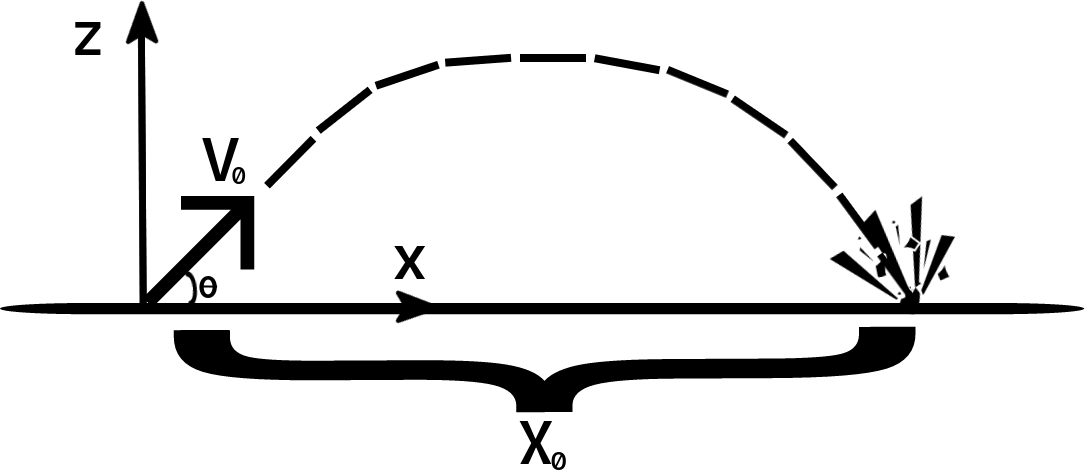
\includegraphics[scale=0.3]{problema3fig1}
\caption{Problema 3}
\label{fig:problema3}
\end{figure}

\vspace{.3cm}

De la (figura \ref{fig:problema3}) utilizando las relaciones trigonométricas en un 
triángulo rectángulo vemos que

\begin{gather*}
v_{0x} = v_0\cos(\theta) \\
v_{0z} = v_0\sen(\theta)
\end{gather*}


Si la partícula de masa $m$ está sujeta a la atracción gravitacional
por la tierra, entonces tenemos, utilizando la segunda ley de Newton,

\vspace{.3cm}

En la dirección de $x$,

\begin{equation}
 0 = m \ddot{x}
 \label{ec:1}
\end{equation}

y en la dirección de $z$,

\begin{equation}
 - mg = m \ddot{z}
  \label{ec:2}
\end{equation}

De la ecuación (\ref{ec:1}) tenemos que (utilizando las condiciones iniciales),

\begin{equation*}
 \ddot{x} = 0 \Rightarrow \frac{d\dot{x}}{dt} = 0 \Rightarrow 
 \int_{v_{0x}}^{\dot{x}}d\dot{x}' = 0 \Rightarrow \dot{x} - v_{0x} = 0 
 \end{equation*}

\begin{equation}
 \therefore \dot{x} = v_0 \cos(\theta)
 \label{eq:3}
\end{equation}

De la ecuación (\ref{eq:3}) podemos obtener $x(t)$, 

\begin{equation*}
 \frac{dx}{dt} = v_0 \cos(\theta) \Rightarrow dx = v_0 \cos(\theta) dt \Rightarrow
 \int_0^x dx' = v_0 \cos(\theta) \int_0^t dt'
\end{equation*}

\begin{equation}
 \therefore x = v_0 t \cos(\theta)
 \label{eq:4}
\end{equation}

Luego para $z$, utilizando la ecuación (\ref{ec:2}),

\begin{equation*}
 \ddot{z} = -g \Rightarrow \frac{d\dot{z}}{dt} = -g \Rightarrow 
 \int_{v_{0z}}^{\dot{z}}d\dot{z}' = -g \int_0^t dt' \Rightarrow \dot{z} - v_{0z} = -gt 
 \end{equation*}
 
\begin{equation}
 \therefore \dot{z} = -gt + v_0 \sen(\theta)
 \label{eq:5}
\end{equation}

De la ecuación (\ref{eq:5}) podemos obtener $z(t)$,

\begin{gather*}
 \frac{dz}{dt} = -gt + v_0 \sen(\theta) \Rightarrow dz = (-gt + v_0 \sen(\theta)) dt \\ \Rightarrow
 \int_0^z dz' = -g\int_0^t t' dt' + v_0 \cos(\theta) \int_0^t t'dt'
\end{gather*}

\begin{equation}
 \therefore z = - g \frac{t^2}{2} + v_0 t \sen(\theta)
 \label{eq:6}
\end{equation}

Podemos encontrar el rango máximo de distancia que recorrerá el proyectil, 
es decir hasta que choque con el piso, cuando llegue al punto que hemos llamado
$x_0$, lo cual ocurre al final de su recorrido cuando $z=0$. Para dar
respuesta a la parte $a)$ de la pregunta debemos determinar en qué momento
esto ocurre, es decir cuánto es el valor del tiempo para el punto en que 
$z=0$, ya que esto nos permitirá determinar los ángulos de lanzamiento
que requerimos para que el proyectil llegue a $x_0$ y $z=0$.

\vspace{.3cm}

Debido a que el proyectil sale disparado desde el origen, $z=0$ cuando
$t=0$, pero mediante la ecuación (\ref{eq:6}) podemos determinar el otro
momento en que $z=0$ que es al final de su recorrido, y a este tiempo
lo llamaremos $\tau$, reescribiendo (\ref{eq:6}) podemos ver esto claramente,

\begin{equation*}
 z = t(\frac{-gt}{2} + v_0 \sen(\theta)) = 0
\end{equation*}

Donde vemos que $z=0$ si $t=0$, pero también para un tiempo $\tau$,

\begin{equation*}
 \frac{-g\tau}{2} + v_0 \sen(\theta) = 0
\end{equation*}

Resolviendo para $\tau$,

\begin{equation}
 \tau = \frac{2v_0\sen(\theta)}{g}
 \label{eq:7}
\end{equation}

Entonces para obtener el rango del proyectil en $z=0$ cuando
$t=\tau$, sustituimos en (\ref{eq:4})

\begin{equation*}
 x = v_0 \tau \cos(\theta) \Rightarrow x = 2 \frac{(v_0)^2}{g} \sen(\theta)\cos(\theta)
\end{equation*}

Utilizando la identidad trigonométrica $2\sen(\theta)\cos(\theta) = \sen (2\theta)$,
obtenemos que

\begin{equation}
 x = \frac{(v_0)^2}{g} \sen(2\theta)
 \label{eq:8}
\end{equation}

El rango será máximo, es decir el proyectil llegará a $x_0$ y $z=0$ para
la familia de ángulos $\theta$ que hagan que $\sen(2\theta)=1$, tales
ángulos son:

\begin{equation}
 \theta = \frac{n\pi}{4} \qquad \qquad n = 4\epsilon - 3, \quad  \epsilon = 1,2,3,4,5,\dots
 \label{eq:9}
\end{equation}

















\vspace{.3cm}

4.- Dos partículas de masa $m_1$ y $m_2$ están amarradas por una cuerda sin masa de 
longitud $l$ y descansan sobre una mesa sin fricción. En el instante t=0 la cuerda
está totalmente desplegada y las masas están en reposo; en ese instante se le aplica
un impulso a la partícula $m_2$ de tal suerte que ésta adquiere una velocidad $v_0$ 
perpendicular a la cuerda.

\begin{enumerate}[a)]
 \item Describa el movimiento después de haber aplicado el impulso
 \item ¿Cuál es la tensión de la cuerda durante el movimiento?
\end{enumerate}

\vspace{.3cm}

\underline{Solución:}

\vspace{.3cm}

5.- Una partícula de masa $m_1$ tiene una energía cinética $T_1i$ y choca elásticamente 
con otra de masa $m_2$. La segunda partícula sale disparada en una dirección que hace un
ángulo $\theta$ con la dirección del movimiento inicial de la primera partícula. Encuentre
la energía cinética $T_2f$ con la que sale la segunda partícula. Muestre que esta energía
es máxima si el choque es de frente.

\vspace{.3cm}

\underline{Solución:}

\vspace{.3cm}

Para la resolución de este problema se seguirán las convenciones y notación de \cite{marion} y algunos
otros autores para el tratamiento de las colisiones elásticas. Como dicen los autores, 
la descripción de muchos procesos físicos puede simplificarse considerablemente, si se 
escoge un sistema de coordenadas en reposo con respecto al centro de masa del sistema. Según
el enunciado del problema puede asumirse que la segunda partícula estaba en reposo, mientras
que la primera va directo a chocarla. Las mediciones reales se hacen en el sistema de coordenadas
del laboratorio en el cual el observador está en reposo, en este sistema una de las partículas
está en movimiento, mientras que la otra está en reposo. No tenemos la misma imagen desde el
sistema de coordenadas del centro de masa como veremos más adelante. Denominaremos al primero como el sistema \textbf{LAB}
y al segundo como el sistema \textbf{CM}.


\vspace{.3cm}

Usaremos la siguiente notación:

 \begin{gather}
 \begin{split}
% 
  m_1 = \text{Masa de la partícula en movimiento} \\
  m_2 = \text{Masa de la partícula en reposo}
%  
  \label{eq:masas}
%  
 \end{split}
 \end{gather}

Usaremos cantidades con primo (') para el sistema CM,

 \begin{gather}
 \begin{split}
  u_1 = \text{Velocidad inicial de } m_1 \text{en el sistema LAB} \\
  v_1 = \text{Velocidad final de } m_1 \text{en el sistema LAB} \\
%   
  u_1' = \text{Velocidad inicial de } m_1 \text{en el sistema CM} \\
  v_1' = \text{Velocidad final de } m_1 \text{en el sistema CM}
% 
 \label{eq:velMasa1}
 \end{split}
 \end{gather}

  \begin{gather}
  \begin{split}
   u_2 = 0 \\
   v_2 = \textrm{Velocidad final de} m_2 \textrm{en el sistema LAB} \\
%  
 \vspace{.2cm}
%  
  u_2' = \textrm{Velocidad inicial de} m_2 \textrm{en el sistema CM} \\
  v_2' = \textrm{Velocidad final de} m_2 \textrm{en el sistema CM}
%  
  \label{eq:velMasa2}
  \end{split}
 \end{gather}
 
También para las energías cinéticas,
 
 \begin{gather*}
  T_0 = \textrm{Energía cinética total inicial en el sistema LAB} \\
  T_0' = \textrm{Energía cinética total inicial el sistema CM} \\
%  
%  
   T_{1i} = \textrm{Energía cinética inicial de } m_1 \textrm{en el sistema LAB} \\
   T_{1i}' = \textrm{Energía cinética inicial de } m_1 \textrm{en el sistema CM} \\
%   
   T_{2i} = \textrm{Energía cinética inicial de } m_2 \textrm{en el sistema LAB} \\
   T_{2i}' = \textrm{Energía cinética inicial de } m_2 \textrm{en el sistema CM} \\
%  
  T_{1f} = \textrm{Energía cinética final de } m_1 \textrm{en el sistema LAB} \\
  T_{1f}' = \textrm{Energía cinética final de } m_1 \textrm{en el sistema CM} \\
%  
  T_{2f} = \textrm{Energía cinética final de } m_2 \textrm{en el sistema LAB} \\
  T_{2f}' = \textrm{Energía cinética final de } m_2 \textrm{en el sistema CM} \\
%
\label{eq:energiasCineticas}
  \end{gather*}

Llamaremos $\textbf{V}$ a la velocidad del centro de masa en el sistema LAB, $\psi$ al 
ángulo en que $m_1$ se desvía en el sistema LAB, $\xi$ al ángulo en que $m_2$ se desvía
en el sistema LAB y $\theta$ al ángulo en el que $m_1$ y $m_2$ se desvían en el sistema CM.

De acuerdo con la definición de centro de masa, tenemos que

\begin{equation}
 m_1 \mathbf{r_1} + m_2 \mathbf{r_2} = M\mathbf{R}
 %
 \label{eq:CM1}
\end{equation}

Diferenciando (\ref{eq:CM1}) con respecto al tiempo encontramos

\begin{equation}
 m_1 \mathbf{u_1} + m_2 \mathbf{u_2} = M\mathbf{V}
 \label{eq:CMVel1}
\end{equation}

Pero debido a que $\mathbf{u_2}=0$ y que $M=m_1+m_2$, el centro de masa se mueve
hacia $m_2$ con una velocidad,

\begin{equation}
\mathbf{V} = \frac{m_1 \mathbf{u_1}}{m_1+m_2}
 \label{eq:CMVel2}
\end{equation}

Debido a que $m_2$ está en reposo al inicio, la velocidad inicial de $m_2$ en el sistema
CM debe ser igual a $V$:

\begin{equation}
u_2'= V = \frac{m_1 u_1}{m_1+m_2}
 \label{eq:u2iniVel}
 \end{equation}
  
Pero notando que el movimiento y las velocidades son opuestas en dirección, i.e. $\mathbf{u_2'=-\mathbf{V}}$.
En el sistema CM, de la manera en que lo hemos escogido, el momentum lineal total es cero, por lo tanto
antes de la colisión las partículas se mueven la una hacia la otra, y luego de la colisión
se mueven exactamente en direcciones opuestas. Debido a que la colisión es elástica,
las masas no cambian, y la conservación del momentum y la energía cinética son suficientes
para decirnos que la velocidad en el sistema CM son iguales antes y después de la colisión,
por lo que 

\begin{equation}
 u_1'=v_1', \quad u_2'=v_2'
 \label{eq:velIguales}
\end{equation}

De (\ref{eq:u2iniVel}) vemos que 

\begin{equation}
v_2'= \frac{m_1 u_1}{m_1+m_2}
 \label{eq:u2finalVel} 
\end{equation}

Recordando la forma expresar las velocidades en el sistema LAB con respecto al centro de masa,
tomando como ejemplo una velocidad arbitraria $v_x$

$$
v_{x,LAB} = v_{x,CM} + v_{CM,LAB}
$$

Tenemos entonces que, utilizando nuestra notación y la ecuación (\ref{eq:u2iniVel}),

\begin{equation}
 u_1 = u_1' + V = u_1' + u_2'
 \label{eq:u1iniVel}
\end{equation}

Utilizando las ecuaciones (\ref{eq:velIguales}) y (\ref{eq:u1iniVel}), podemos ver entonces que 

 \begin{gather}
 \begin{split}
% %
   v_2' = \frac{m_1 u_1}{m_1 + m_2} \\
%   %
   v_1' = u_1 - u_2' = \frac{u_1 m_1 + \cancel{m_2 u_1} - \cancel{m_2 u_1}}{m_1 + m_2} =
   \frac{m_2 u_1}{m_1 + m_2}\\
%   %
   \label{eq:velFinales}
%   %
 \end{split}
 \end{gather}

Ya estamos en posición entonces para encontrar expresiones y relaciones que involucren
la energía de las partículas. En el sistema LAB y debido a que la colisión es elástica,
la energía cinética total inicial es igual a la energía cinética de la partícula $m_1$,
es decir

\begin{equation}
 T_0 = \frac{1}{2} m_1 u_1^2
 \label{eq:energCinetTotIniLAB}
\end{equation}

y en el sistema CM,


\begin{equation}
 T_0' = \frac{1}{2} (m_1 u_1'^2 + m_2 u_2'^2)
 \label{eq:energCinetTotIniCM1}
\end{equation}

pero utilizando las expresiones para las velocidades de (\ref{eq:velFinales}), 
la ecuación (\ref{eq:energCinetTotIniCM1}) se convierte en 

\begin{align}
\begin{split}
 %
 T_0' &= \frac{1}{2} \left[ \left(\frac{m_1 u_1}{m_1 + m_2}\right)^2 + m_2 \left(\frac{m_2 u_1}{m_1 + m2+}\right)^2\right] \\
 %
       &= \frac{1}{2} \left[ u_1^2 \frac{m_1 m_2^2}{(m_1+m_2)^2} + u_1^2 \frac{m_2 m_1^2}{(m_1+m_2)^2}\right] \\
%  %
       &= \frac{1}{2} \left[ m_1 m_2 u_1^2 \left( \frac{m1}{(m_1 + m_2)^2} + \frac{m_2}{(m_1 + m_2)^2}\right)\right] \\
%  %
       &= \frac{1}{2} \left[ m_1 m_2 u_1^2 \left( \frac{m_1+m_2}{(m_1+m_2)^2}\right) \right] \\
%  %
       &= \frac{1}{2} \left( \frac{m_1 m_2}{m_1+m_2}u_1^2 \right) \\
%  %
\therefore T_0' &= \frac{m_2}{m_1+m_2} T_0
 %
\end{split}
\end{align}

El problema nos pide cual es la energía cinética $T_{2f}$ con la que sale la segunda partícula,
ya con los resultados que hemos obtenido es fácil obtener la misma, calcularemos
la energía cinética final de la partícula $m_1$ y $m_2$ tanto para el sistema
LAB como para el sistema CM, para ello utilizando las expresiones para las 
velocidades finales de la ecuación (\ref{eq:velFinales}),

\begin{align}
\begin{split} 
%
 T_{1f}' &= \frac{1}{2} v_1'^2 \\
 %
	 &= \frac{1}{2}m_1\left(\frac{m_2}{m_1+m_2}\right)^2 u_1^2 \\
	 %
	 &= \left(\frac{m_2}{m_1+m_2}\right)^2 T_0\\
%
\label{eq:erergCineFinalm1CM}
\end{split}
\end{align}

y

\begin{align}
\begin{split} 
%
 T_{2f}' &= \frac{1}{2} v_2'^2 \\
%
	 &= \frac{1}{2}m_2\left(\frac{m_2}{m_1+m_2}\right)^2 u_1^2 \\
%
	 &= \frac{1}{2}m_1 u_1^2 \frac{m_1 m_2}{(m_1+m_2)^2} \\
%
	 &= \frac{m_1 m_2}{(m_1+m_2)^2} T_0
%
\label{eq:erergCineFinalm2CM}
\end{split}
\end{align}







6.- Un objeto de masa $m$ se encuentra en el ecuador de la Tierra. ¿Qué velocidad debe 
tener para que su peso y la fuerza de Coriolis sean iguales?

\vspace{.3cm}

\underline{Solución:}

\vspace{.3cm}

El efecto de la rotación de la Tierra sobre los experimentos de laboratorio es muy pequeño, pero sin embargo se puede
hacer un tratamiento del problema planteado considerandolo como un problema de movimiento con respecto
a unsistema de coordenadas en rotación. No demostraremos todas las ecuacioens debido a que se haría
muy larga la solución, pero podemos comenzar por escribir la siguiente ecuación,

\begin{equation}
 \mathbf{F'} = \mathbf{F} - 2m(\mathbf{\omega} \times \mathbf{v'}) - m\mathbf{\omega} \times (\mathbf{\omega} \times \mathbf{r'})
 \label{eq:FuerzasDeSistemaRotacion}
\end{equation}

Donde $\mathbf{F'} = m\mathbf{a'} = d\mathbf{p'}/dt$ es la fuerza que mediría un observador $S'$ situado
en un sistemas de coordenadas en rotación, $\mathbf{F}$ es la fuerza que mediría un observador
en reposo en un sistema inercial. Los dos términos resultantes son las conocidas \emph{fuerzas de inercia}:

\begin{equation}
 \mathbf{F_i'} = - 2m(\mathbf{\omega} \times \mathbf{v'}) - m\mathbf{\omega} \times (\mathbf{\omega} \times \mathbf{r'})
 \label{eq:FuerzasDeInercia}
\end{equation}

Donde recordamos que $\mathbf{\omega}$ es la velocidad angular del sistema en rotación. Es evidente que cuando $\mathbf{\omega} = 0$
entonces $S'$ no gira y ambos observadores deberían concordar en las fuerzas. Estas dos fuerzas tienen nombre, el segundo de los términos
recibe el nombre de fuerza centrífuga, aunque no diremos mucho más de ella, cabe resaltar que esta siempre dirigida hacia
afuera, es siempre perpendicular al eje de rotación y es proporcionala $\omega^2$ y a la deistancia al eje.

\vspace{.3cm}

La fuerza que nos interesa para resolver este problema es el primer término de (\ref{eq:FuerzasDeInercia}), $- 2m(\mathbf{\omega} \times \mathbf{v'})$,
llamada \emph{fuerza de Coriolis}, esta como se puede ver depende de la velocidad en $S'$, pero no de la posición. La fuerza de Coriolis 
es perpendicular a $\mathbf{\omega}$ y a $\mathbf{v'}$. En el problema se nos pregunta qé velocidad debe tener un objeto de masa $m$ para que su peso 
y la fuerza de Coriolis sean iguales. Como hemos dicho el efecto de la fuerza Coriolis sobre el movimiento de los cuerpos en la Tierra 
suele ser muy pequeño. Debido a la forma y estructura de la ecuación para la fuerza Coriolis podemos predecir que el objeto se deberá mover 
relativamente rápido para que su peso y la fuerza de Coriolis sean iguales, porque la velocidad angular de la tierra es de unos $2\pi$ 
radianes por día sideral (23 $h$, 56 $m$, 4.1 $s$) lo que da un valor aproximado de $7.3 \times 10^-5$ rad/s. El hecho de que el
cuerpo está en el ecuador facilita un poco el cálculo ya que no hay que considerar las correcciones para la fuerza Coriolis en el
hemisferio norte o sur de la Tierra.

\vspace{.3cm}

Entonces lo que requerimos es que para el objeto de masa $m$ se cumpla

\begin{equation}
 - 2m(\mathbf{\omega} \times \mathbf{v'}) = - m \mathbf{g}
 \label{eq:Coriolis1}
\end{equation}

De (\ref{eq:Coriolis1}), la velocidad que debe tener el cuerpo es de (asumiendo que se encuentra a nivel del mar
y una distribución homogénea del campo gravitacional que lo afecta)

\begin{equation}
 \boxed{ v' = \frac{g}{2\omega} = \frac{9.8 m/s^2}{7.3 \times 10^-5 rad/s} = 6.72 \times 10^5 m/s}
\end{equation}


\vspace{.3cm}

7.- La hélice de un avión tiene un momento de inercia $I$ y el motor le imprime una torca 

$$N_m = N_0 (1+\alpha \cos{\omega t}. \qquad (\alpha \ll 1))$$

La resistencia del aire le imprime una torca

$$N_f = -b\dot{\theta}$$

¿Cuál es el estado estacionario del movimiento de la hélice?

\vspace{.3cm}

\underline{Solución:}

\vspace{.3cm}

8.- Dos cuerpos rígidos extensos (no puntuales) chocan elásticamente. ¿Es posible que 
después del choque ambos queden únicamente con energía cinética de rotación en torno 
a sus centros de masa?. De ser así de un ejemplo.
\vspace{.3cm}

\underline{Solución:}

\vspace{.3cm}
9.- Un meteorito choca con la Tierra en el Polo Norte haciendo un ángulo $\theta$ con
el eje de la tierra. El meteorito tiene una masa igual a $1/10^-17$ de la masa de la 
Tierra y llega con la velocidad de escape. ¿En qué forma se verá perturbado el movimiento
de rotación de la Tierra? (Desprecie el cambio en el momento de inercia de la Tierra
debido a la incrustación del meteorito).
\vspace{.3cm}

\underline{Solución:}

\vspace{.3cm}

10.- Uno de los postulados básicos de la mecánica clásica es el de la relatividad galileana,
nos dice que la mecánica clásica debe ser invariante ante las transformaciones de Galileo, 
esto es las leyes de la física básica deben ser las mismas en todos los sistemas inerciales
de referencia y la transformación entre un sistema inercial y otro es la de Galileo 
($\hat{r}' = \hat{r} - \hat{v}'t$ donde $\hat{v}'$ es la velocidad constante entre los dos 
sistemas de referencia).

\begin{itemize}
 \item En la formulación de Newton de 1687 se consideraba la existencia de un sistema 
 absoluto de referencia que permitía definir el estado de reposo de un cuerpo, Newton lo
 veía como un sistema anclado a las estrellas fijas o uno muy cercano a este. La visión 
 moderna se desarrolló en el siglo XIX, elimina la idea del reposo absoluto y hace 
 uso del postulado que mencionamos. Describa brevemente el cambio entre la visión 
 estrictamente newtoniana y la del siglo XIX.
 \item Muestre, a manera de ejemplo del cumplimiento del postulado anterior, que las 
 ecuaciones de movimiento del oscilador armónico tridimensional son invariantes ante
 las transformaciones de Galileo.
\end{itemize}

\vspace{.3cm}

\underline{Solución:}

\vspace{.3cm}

\begin{thebibliography}{10}
 \bibitem{marion}
 S. Thronton y J. Marion, \textit{Classical dynamics of particles and systems}, Thomson Brooks/Cole,
 5ta edición, 2004.
 \bibitem{taylor}
 J. Taylor, \textit{Classical mechanics}, University Science Books, 2005.
 \bibitem{zill}
 D. Zill y W. Wright, \textit{Differential equations with Boundary-Value Problems}, Brooks/Cole,
 8va edición, 2013.
\end{thebibliography}


\end{document}
